\documentclass[output=paper]{langsci/langscibook}
\author{Robin Clark\affiliation{University of Pennsylvania}}
\title{Drift, finite populations, and language change}

% \chapterDOI{} %will be filled in at production

\abstract{History happens only once. This seems to set up an impenetrable
    barrier for social sciences, like historical linguistics,  that concern
    themselves with change over time.  We have the historical record to go on
    with no convincing way to generate alternative histories that could be used
    for hypothesis testing. Nevertheless, it is of some interest to ask whether
    what we see in the historical record is due to particular forces or whether
    the time series we see could be the result of random drift.  In this paper,
    I will spell out some simple principles of random drift that can be used to
    construct  null hypotheses against which we can study particular cases of
    \isi{language change}.  The study of random drift allows us to sharpen our
    analyses of \isi{language change} and develop more constrained theories of
    language variation and change.}

\maketitle

\begin{document}\glsresetall

\section{Introduction}

More years ago than I like to count, Ian Roberts and I wondered about the
causal mechanisms of \isi{language change} \citep{clark-roberts:1993}.  At the time,
the idea was that \isi{language change} would happen when the learner cannot uniquely
determine the grammar on the basis of linguistic evidence; in these
circumstances, the learner would be inexorably driven toward the simpler
analysis and the language would change.  I can confess here that my own
thinking about how this could happen was rather thin; I supposed that language
contact, whether between different language groups or different sociolinguistic
levels, would introduce ambiguities into the learner's evidence, thus driving
change.

While there is no doubt that language contact is an important driver of
language change, we should ask whether it is the \emph{sole} driver of change.
Suppose we conclude that language contact is the sole driver of change; what
are we to say about language diversity?  Where does the diversity of languages
come from, if not from multigenesis?  Imagine, though, that a homogeneous
linguistic group is isolated for a millennium; would the language really remain
unchanged over that time, simply because the group had no contact with any
other group?

Clearly, it is worth our while to investigate other potential sources for
language change beyond the clear case of language contact. I will make the
case, here, that random processes (drift) could be a source of \isi{language change}.
More precisely, the sampling error that arises from each individual's
particular experience with language could be a source of language variation,
particularly when amplified through a hierarchical social structure that
includes language leaders, individuals who are taken as models by other members
of their social group.  In fact, as we shall see, this sort of variation is
inevitable in finite populations, a fact that has long been known in population
genetics \citep{crow-kimura:1970}.

\section{Random processes and neutral models}

The Hardy--Weinberg model, an early model of gene frequencies in populations,
had a simple structure that made it an appealing and simple model of change
over time; the equation underlying the model is exceedingly friendly and has
not only been used in biology but has also been usefully adapted to build
mathematical models of social and cultural evolution
\citep{boyd-richerson:1985}, since it can neatly express the relationship
between two variant forms, $p$ and $q$.\footnote{See also
    \citet{llcs-feldman:1981}, one of the earliest attempts to propose a
    population-based model of cultural evolution; \citet{mcelreath-boyd:2007}
is a good overview of mathematical models of social evolution, in particular
their Chapter 1.} From a linguistic perspective, we could take $p$ and $q$ to
be the probability of two linguistic variants that cannot be expressed
simultaneously and are, thus, in competition with each other; for example, $p$
might be the likelihood of verb raising, while $q$ is the probability of
leaving the verb in situ.  In this case, of course, we would take $q$ to be $1
- p$.

Crucially, the model makes a number of assumptions about populations.
First, there is random pairing; individuals do not ``clump'' together
into groups depending on their preference for $p$ or $q$. Second, it
is assumed that selection is not operating on the population; in other
words, one variant is not preferentially replicated.  Third, mutation
and migration are absent; new variants are not introduced that might
compete with the existing options and there is no outflow or inflow of
new variants. Thus, the model in its simplest form would put aside
both innovation (mutation) and language contact (migration) as sources
of change.  Finally, and this point is crucial, the population is
infinite in size so that frequencies of the variants are not subject
to chance fluctuations.\footnote{The literature on the Hardy--Weinberg
  model is extensive.  \citet{bergstrom-dugatkin:2012} contains a
  highly accessible introduction to the mathematics.}  These
assumptions implied that, all else being equal, the population would
quickly achieve a \emph{mixed equilibrium state}.  This means that, in
the absence of selection, the population frequencies for the character
in question would remain stable. The frequencies in a population, if
disturbed, will quickly return to equilibrium.  If, however, some
force acts on the underlying frequencies, then the population will
happily rest at the new frequency.  One such force would be
\emph{selection}, where one variant is, for whatever reason, preferred
over the other.  An observed positive change in frequencies of a
character would then imply that either positive selection was working
on the characteristic or that negative selection was acting on the
other variant of that characteristic.

To make the discussion concrete, suppose that the variants are (1)
inversion of the subject and the main verb in questions or (2)
insertion of an auxiliary\is{auxiliaries} verb which is then inverted with the
subject.  Suppose further that the frequency of the second variant
is increasing.  A Hardy--Weinberg model would treat this as either
selection for the second variant or selection against the first
variant.  Otherwise, in the absence of selection, the relative
frequencies of the two types should remain constant.

Although the model is appealingly simple, population biologists soon
questioned the assumption that the population is infinite. Clearly
infinite populations don't exist in nature, so it's of some interest to
consider what happens in a finite population.  So let's suppose that
we have a finite population of $N$ individuals.  Since we are
interested in the spread of properties in a population, we can safely
suppose that some features are replicated by a copying process.  Since
the population is finite, we can further suppose that some copies are
removed from the population.  More precisely, at each time step, one
individual is randomly selected from the population according to a
uniform distribution and copied and one individual is randomly
selected and deleted.  This is a \emph{Moran process}
\citep{moran:1958}, and it is a simple model of how random forces due
to sampling can act on a population.  This process should have some
resonance in linguistics, since variants might be randomly sampled in
the population; by chance, I may have heard the past tense of
\emph{sneak} as \emph{snuck} rather than \emph{sneaked} and might,
therefore, develop a preference for \emph{snuck}.  In general, because
the process is sampling a finite population, chance becomes an
important force so that large changes in population frequencies could
be due to random factors.  Notice that these random changes can build
up over time, resulting in a change going to completion; no other
forces need to be acting on the population.  Thus, a population will
change over time in the absence of actual selection; see the
discussion of the neutral model, below.

\begin{figure}
  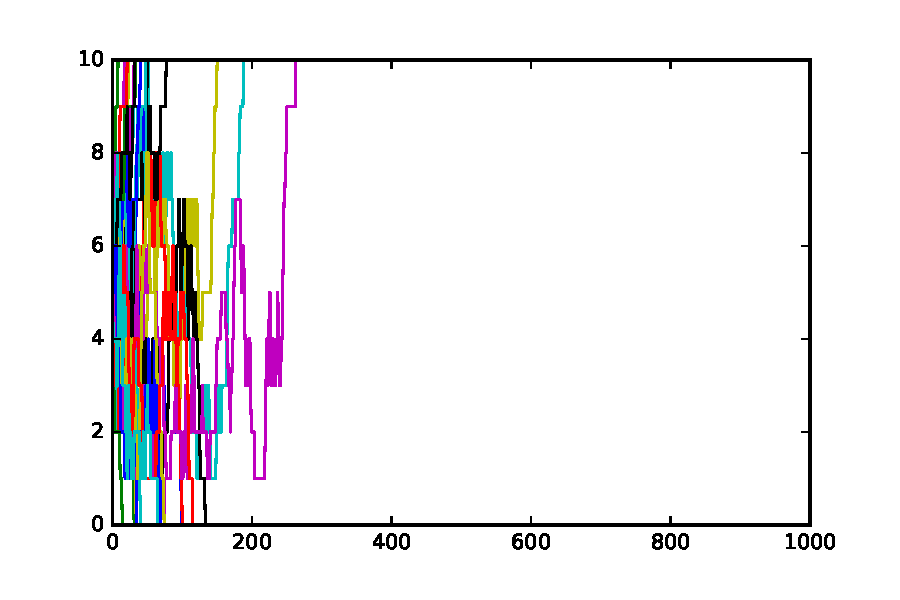
\includegraphics[width=.75\linewidth]{img/pop10_1000.pdf}
  \caption{$N=10$, 1,000 steps, 15 repetitions\label{random_fig1}}
\end{figure}

Figures \ref{random_fig1}--\ref{random_fig3} show the results of three
different experiments with this random process in populations of
various sizes, the process repeated fifteen times for each population
size; in all these cases, we are simply applying the random sampling
process described above to the population.  In all these cases, the
$x$-axis shows the number of steps and the $y$-axis shows the
number of individuals bearing some variable trait, call it
``$A$.''  My interest here is simply to show the potential effects of
population size, so what we will do is consider how this random
process plays out on populations of different sizes, ranging from 10
individuals and going through orders of magnitude.  We will briefly
turn to the applicability to language below.

In \Cref{random_fig1}, the population consists of 10 individuals.
We begin with half the population having the trait $A$ and the other
half lacking it; the figure tracks the frequency of the trait in the
population over time.  By hypothesis, the trait itself has no
consequences for either survival or reproduction.  It is clear from
\Cref{random_fig1} that in a small population whatever the trait
is, it quickly either takes over or is removed from the entire
population.  Since the trait has no consequences for survival or
reproduction, the end result, whether it is fixation or elimination,
is entirely up to chance, a function of random sampling.  Because the
population is so small, a great deal of variation emerges in short
order.  Small populations tend to have higher variance and will more
quickly show the effects of random drift; in this case, a sample size
of one has consequences for 10\% of the population, so it is no wonder
that the variance is so high.  Note that the population quickly
fixates, either with the entire population having $A$ or with $A$
being driven out of the population.  This implies that in small
populations it will be very difficult to distinguish selection for a
trait from simple drift.

\begin{figure}
    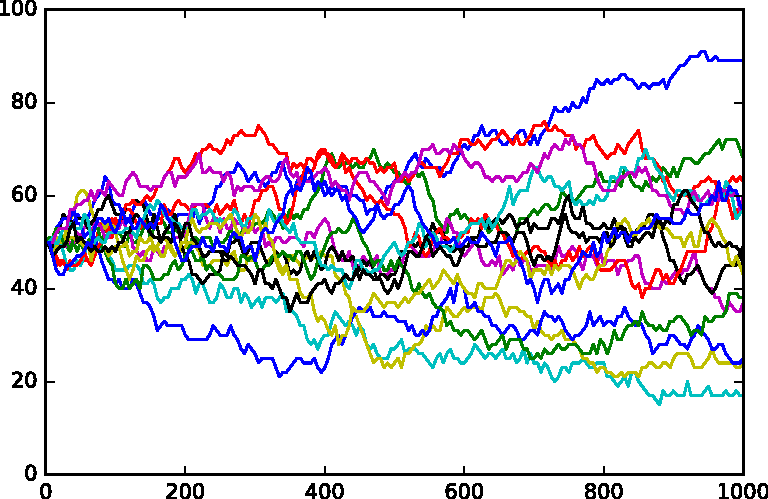
\includegraphics[width=.75\linewidth]{img/pop100_1000.pdf}
    \caption{$N=100$, 1,000 steps, 15 repetitions\label{random_fig2}}
\end{figure}

In \Cref{random_fig2}, the population is an order of magnitude
larger than in the first experiment, with a population size of 100
individuals as opposed to the population of 10 individuals.  Again, we
begin with half of the population having the trait $A$. The figure
tracks the frequency of $A$ over time.  We can see that
variance increases over time, although the increase is slower than in
the small population of 10 individuals.  Despite the fact that the
change in variance is slower than in the smaller population, it is
still considerable after only 1,000 steps; in some repetitions the
trait is present in about 90\% of the population while in others the
trait is present in only about 20\% of the population.  We can be sure
that eventually, the population will eventually go to
\emph{completion}; variation will eventually disappear either when the
entire population has $A$ or when is vanishes from the population; no
middle course is possible \citep{sigmund:1993}.

In \Cref{random_fig3}, I have increased the size of population by
yet another order of magnitude, to 1,000 individuals, and followed the
process for 15 repetitions of 1,000 steps.  With this population, the
variance grows even more slowly relative to the population size.
Nevertheless, it is clear that the variance does grow, as can be seen
by comparing the spread of the population from step 200 to step 1,000.
Indeed, as in the above cases, the population will eventually go to
completion, although it may take a much long time to do so.  It is as
though increases in population size have the effect of increasingly
stretching the diagram in \Cref{random_fig1} while retaining the
outcome: ultimate completion of the change after adequate time.

\begin{figure}
    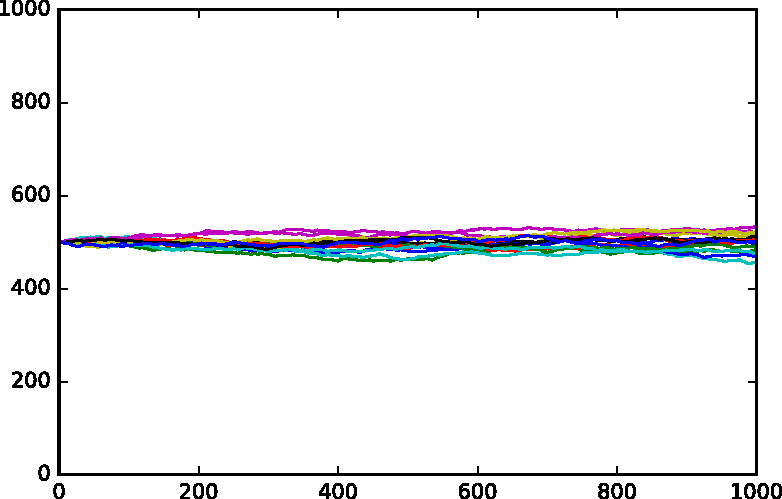
\includegraphics[width=.75\linewidth]{img/pop1000_1000.pdf}
    \caption{$N = 1,000$, 1,000 steps, 15 repetitions\label{random_fig3}}
\end{figure}

While I'm certainly not claiming that \isi{language change} is a Moran
process, these experiments show a number of important features of
finite populations and random sampling.  First, it is clear that
random forces can be a compelling force on populations, one which,
over the long term, can result in large changes in frequencies.
Unlike the simple model on infinite populations, once we have observed
a change in frequency of a trait in a finite population, we must ask
whether that change of frequency can be accounted for solely in terms
of a random force, like sampling error, or whether we must appeal to
selection if we are to understand the change. This point holds for the
time series of frequencies of variant linguistic features as much as
it does for time series of the frequency of genes in a population.
This fact has import consequences for the study of \isi{language change}.

Second, the size of a population plays a crucial role in change; the smaller
the population, the easier it is for chance to buffet the frequencies,
resulting in large short-term changes of frequency of a variant in a small
population.  As the size of the population grows, it will be less likely that
randomness will result in rapid changes in frequency. Thus, if we observe a
rapid change in the frequency of a trait, the larger the population is, the
more likely it is that the change is a result of selection rather than chance.
In a small population, as \Cref{random_fig1} illustrates, precipitous changes
of frequency due to chance are not unusual.

The interpretation of population size with respect to language change
is an important question.  It seems to me unlikely that population,
here, refers to the number of speakers of the language, although there
will clearly be some relation between change and the number of
speakers.  If the relationship were a simple one, then we would expect
languages with more speakers to change more slowly than languages with
smaller numbers of speakers.  I'm inclined to take population to be
more intimately related to the frequencies of the forms in question.
Extremely frequent forms should change only very slowly, while less
frequent forms should be more inclined to drift.  This accords well
with the observation that irregular plural forms in \ili{English} are likely
to be frequent (\emph{foot}/\emph{feet}, \emph{man}/\emph{men},
\emph{child}/\emph{children}, \emph{mouse}/\emph{mice} and so on).\footnote{See
\citet{newberry-etal:2017} for some work on regular and irregular past tense in
American \ili{English}, as well as other changes including periphrastic
\emph{do} and verbal negation.}  These reflect older stages of the language
which retain vestiges of an older system but resisted change to the regular
form by virtue of their ``large population'' (high frequency).  Indeed, casting
our net more widely, we see evidence that high frequency correlates with
stability; highly frequent forms are more stable and retained longer while low
frequency forms are less stable and are not retained as long;  see, for
example, \citet{pagel-etal:2007} on rates of lexical change in Indo-European;
\citet{lieberman-etal:2007} and \citet{newberry-etal:2017} for connections
between word frequency and rates of change for irregular verbs in
\ili{English}.

Third, we want to be able to reliably distinguish changes that are
consistent with random drift from changes that are more likely the
result of selection.  If we are to understand cases of language change
(in particular) and social change (in general), we will want to have
a method of classifying the changes we observe in those that are
consistent with random drift as the sole force of change and those
where we can reject random drift as the sole force.   We cannot
classify cases of change simply by looking at individual curves.

\begin{figure}
    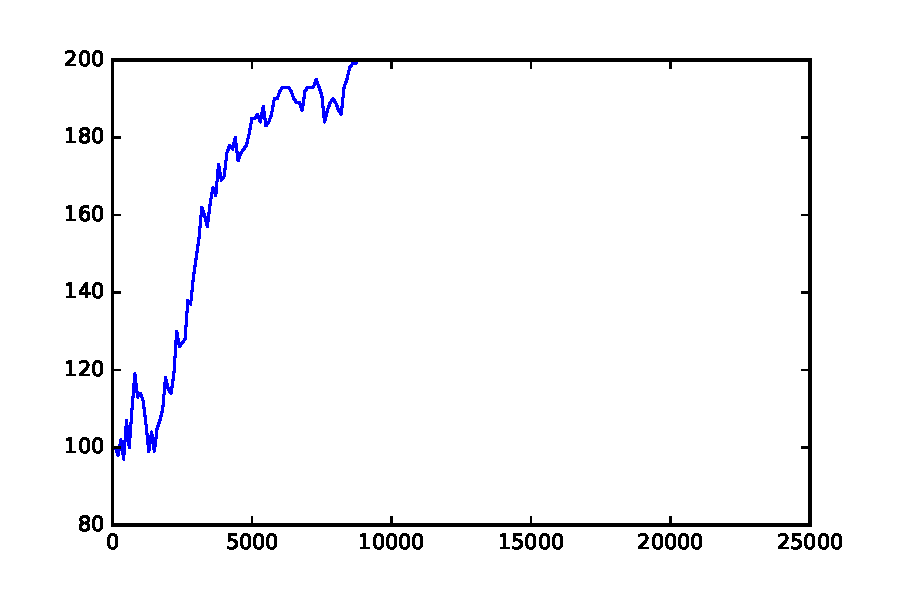
\includegraphics[width=.75\linewidth]{img/result.pdf}
    \caption{$N = 200$; 25,000 steps\label{RandomDrift}}
\end{figure}

Consider the change shown in \Cref{RandomDrift}, which was again
generated by a Moran process.  The curve shows a change in frequency
of a trait for a population of 200 individuals. It looks sigmoidal,
which we would expect if the trait was being selected for, but it was
generated by the same Moran process used in the experiments shown in
Figures \ref{random_fig1}--\ref{random_fig3}; we know that the process
did not involve selection although, by chance, this curve appears to
be nicely sigmoidal.  We cannot reject the hypothesis that a change is
due to chance simply by looking at a curve with the naked eye.  We
need a reliable method that takes into account population size, rates
of change and so forth; the method should, furthermore, have wide
application not only to \isi{language change}, but to the quantitative study
of other types of change so that we can accumulate evidence for the
fundamental scientific reliability of the method.

\begin{figure}
  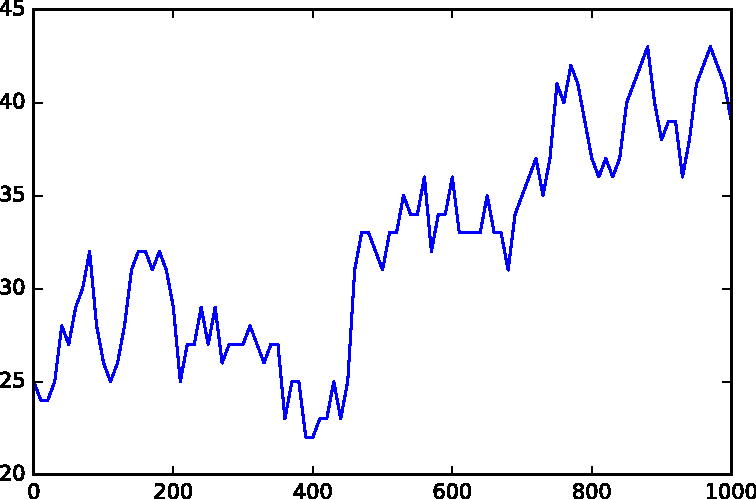
\includegraphics[width=.75\linewidth]{img/jaggedy.pdf}
  \caption{$N = 50$; 1,000 steps\label{jaggedy}}
\end{figure}

Now look at the curve in \Cref{jaggedy}.  This curve was again
generated by a Moran process on a population of 50 individuals.  The
curve ultimately trends toward the trait dominating in the population,
although the frequencies vary up and down in a seemingly random
fashion.  It is common practice to partition the data from historical
corpora into time bins.  In \Cref{smoothed}, I've broken the
frequencies used in \Cref{jaggedy} into quintiles, calculated
the average in each quintile and graphed the result.  The new curve
shows an initial decline in the trait ``A'' followed by an apparently
smooth monotonic increase that could be selection; the curve is
clearly sigmoidal.  Of course, we know that the underlying process was
simply random sampling of a small population.

\begin{figure}
  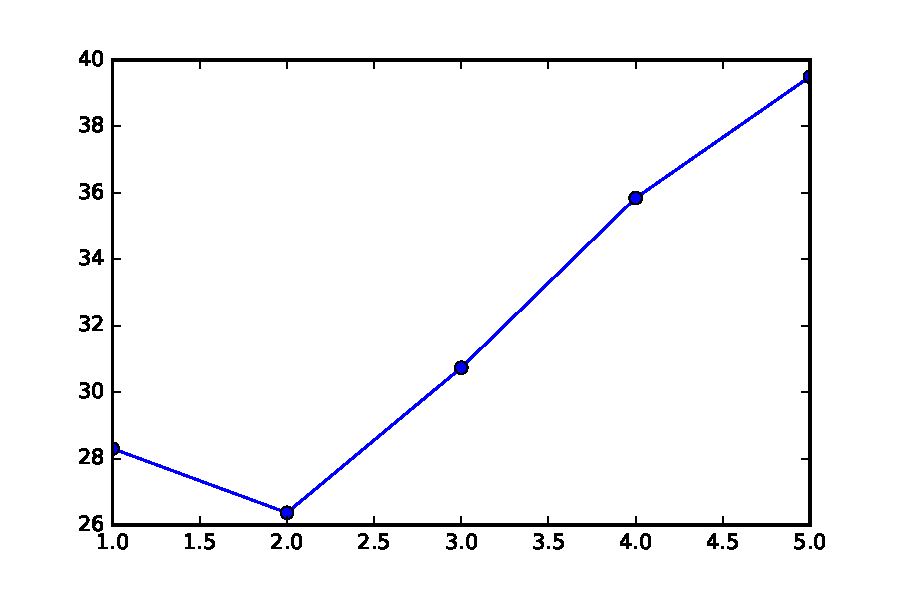
\includegraphics[width=.75\linewidth]{img/smooth_data.pdf}
  \caption{Average frequencies of quintiles\label{smoothed}}
\end{figure}

%Below we will
%discuss the application of the methods developed by
% to \isi{language change}.

This brings up an important point.  Random processes are always at
work during evolutionary change \citep{kimura:1983}.  Thus, when we
see a change of frequency of a trait in a time series, we need to ask
whether or not this change could be due to selection or whether that
change is consistent with random drift.  If we can rule out drift for
a particular bit of \isi{language change}, we can then ask why that trait
was selected for (or, for that matter, against).  Factors might
include properties of sentence processing, learnability, or social
factors (social networks, prestige, or identity).  Note that we are
not claiming that drift is a theory of \isi{language change} by itself but,
rather, that random processes are everpresent and must be controlled
for in developing a theory of \isi{language change} or, more broadly, social
and cultural evolution.

A theory of the random processes associated with \isi{language change} would
provide a \emph{neutral model} of language, one where changes in
frequency are solely due to stochastic processes.  We could then
compare the statistical properties of a given change with the
predictions of the neutral model.\footnote{Recently, neutral models
  have begun to receive a great deal of attention, long overdue.  See
  \citet{baxter-etal:2006, baxter-etal:2009, blythe:2012,
    blythe-croft:2012, kauhanen:2017, stadler-etal:2016} for an array
  of approaches.} In \citet{newberry-etal:2017}, we tested
drift by using techniques developed by \citet{feder_etal:2014}; the
essential idea is relatively straightforward.  Suppose we have a time
series of frequencies of some variable trait. Starting at zero, we can
keep a running sum by adding 1 if the frequency of the trait at a time
step increases and subtracting 1 if the frequency goes down.  We
expect that the sums for drift should show a Gaussian distribution
around 0.  Indeed, we can estimate population size and test whether we
can reject drift for various population
sizes. \citet{newberry-etal:2017} apply the technique to a
number of different time series and argue that not only can we
distinguish between drift and selection, but that we can quantify the
strength of selection relative to population size.  The method should,
when applied to a broad array of different time series data, allow us
to refine our theory of diachronic change.

So far, the reader may think that drift is a problem for the theory of language
change; in fact, though, drift may also help us to understand how language
variation can arise in the absence of language contact.  If the population is
finite, then random processes will guarantee that the variance will increase
with time, as we have seen in our discussion of Moran processes around Figures
\ref{random_fig1}--\ref{random_fig3}.  This, in turn, guarantees that new
variants will constantly be brought into the population.  In other words,
variation can arise in the absence of language contact.

\citet{clark-kimbrough:2015} develop a simple mechanical model of
language variation using a version of exemplar theory
\citep{murphy:2002}. The agents adapt their behavior by finding the
centroid of a set of exemplars (in this case, a set of vowel
pronunciations).  If no other force is acting on the model, then the
agents gradually find the same centroids.  If, however, the model has
more social structure, where some agents are designated as
particularly influential, so that their productions are given extra
weight by other agents, the variance grows enormously. The influential
utterances, in fact, reduce the effective population size
\citep{crow-kimura:1970}, since so many agents tend to imitate these
utterances; in other words, social structure makes the population
smaller, causing a large increase in the variance over time.  This is,
again, an example of how variation can arise spontaneously due to the
statistical properties of small populations.

I began this chapter by recalling a puzzle that Ian Roberts and I had
pondered years ago.  We could see that language contact could trigger
language change; I couldn't quite see how languages would change in
the absence of contact, but surely (I thought) that must be possible.
I now offer a hypothesis about another possible origin for language
variation and \isi{language change}: finite populations. I hope in future
that we will be able to explore this hypothesis with empirical work in
corpora, modeling with Agent-Based Models and experimental laboratory
work.

{\sloppy
\printbibliography[heading=subbibliography,notkeyword=this]
}

\end{document}
